\chapter{Stand van zaken}
\label{ch:stand-van-zaken}
% Tip: Begin elk hoofdstuk met een paragraaf inleiding die beschrijft hoe
% dit hoofdstuk past binnen het geheel van de bachelorproef. Geef in het
% bijzonder aan wat de link is met het vorige en volgende hoofdstuk.

% Pas na deze inleidende paragraaf komt de eerste sectiehoofding.
Niet alles wat in dit onderzoek al is aangekaart, is gemakkelijk te begrijpen. Want natuurlijk zijn de begrippen zoals \emph{Kafka} en \emph{RabbitMq} niet voor iedereen even duidelijk. Ook de term microservices zal bij sommigen de wenkbrauwen wel eens doen fronsen. In dit hoofdstuk is de bedoeling uit te leggen wat al deze begrippen betekenen. Elke tussentitel zal op zijn beurt uitleggen wat een begrip nu eigenlijk is. Na dit hoofdstuk zul je in staat zijn om met deze informatie te begrijpen wat er allemaal gebeurd in dit onderzoek.
\section{Microservices}

Microservices is een software architectuur. De applicatie bestaat uit meerdere kleinere componenten die samen één groot geheel vormen. Deze kleinere componenten zijn onafhankelijk van elkaar en hebben elk hun eigen proces. Deze software architectuur is vrij recent en is de laatste jaren een echte hype aan het worden.

Een belangrijke vraag is: waarom zijn microservices ontstaan? Server-side applicaties gebruiken meestel object-georiënteerde programmeer talen. Deze programmeertalen hebben abstracties om de complexiteit van hun programma's te behandelen in modules. Dit wordt ook wel eens `the monolith` genoemd. Dit is één groot geheel die meestal uit drie lagen bestaat. De presentatielaag, de businesslaag en de datalaag. Deze lagen kunnen niet apart van elkaar gebruikt worden omdat ze verschillende resources met elkaar delen. Dit zorgt ervoor dat bij iedere wijziging in de applicatie, alle lagen opnieuw gereleased worden in een nieuwere versie. Je kan natuurlijk al raden dat dit in een grote applicatie niet de beste oplossing is. 

\begin{figure}[h!]
    \centering
    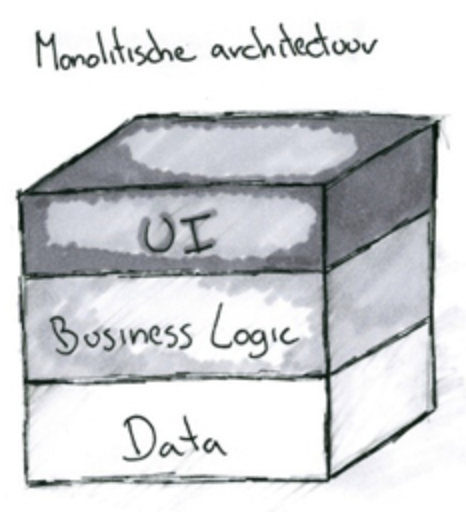
\includegraphics[width=80mm]{../monolith.png}
    \caption{Monolitische architectuur}
        
\end{figure}

Daarom is er een andere architectuur die een heel andere aanpak heeft, namelijk microservices. Dit bestaat uit verschillende kleinere componenten die indien nodig onafhankelijk van elkaar uitgevoerd kunnen worden. Bij deze aanpak is ook belangrijk dat je uw services klein houdt. Hierdoor kunnen je services gemakkelijk hergebruikt, begrepen en opnieuw gebuild worden. Iedere microservice heeft dus maar 1 verantwoordelijkheid.

Omdat microservices op verschillende machines moeten kunnen draaien, bijvoorbeeld op verschillende besturingssystemen, is het beter om ze in te pakken samen met hun dependencies in een container. \emph{Docker} is een voorbeeld van een technologie die deze containers aanbiedt. Door microservices in containers te plaatsen, zorg je ervoor dat de uitvoering van deze services onafhankelijk gebeurd met andere applicaties op dezelfde machine. Containers zijn dus onafhankelijk van een besturingssysteem, hierdoor kunnen microservices op verschillende locaties gedraaid worden. Een van de voordelen hiervan is dat ze door containers in de cloud kunnen geprogrammeerd worden.

De vier grootste voordelen van microservices zijn: 
\begin{itemize}
    \item Schaalbaarheid
    \item Beperken complexiteit
    \item Verkorten time-to-market
    \item Autonomie van ontwikkelteams.
\end{itemize}



 \autocite{Claudio2017} en \autocite{Velthoven2016}

\section{Kafka}

Wanneer je als bedrijf veel berichten binnen krijgt op een korte tijdsspanne, dan heb je natuurlijk een goed functionerende technologie nodig die al deze berichten kan verwerken. \emph{Kafka} is een voorbeeld van zo een technologie. Het is dus een berichtensysteem waarbij schaalbaarheid en redundantie een grote troef zijn. Bepaalde kernwoorden zijn belangrijk om de architectuur van \emph{Kafka} te begrijpen. Deze kernwoorden zijn: topics, producers, consumers en brokers.  

Topics zijn, zoals de naam al doet vermoeden, verschillende onderwerpen. Alle berichten zijn gegroepeerd in een van deze topics. Het formaat van een bericht kan verschillend zijn. Het type kan een gewone tekst zijn, kan van een Json-formaat zijn, of kan iets helemaal anders zijn. Het is mogelijk om zowel naar een specifieke topic een bericht te verzenden als te ontvangen. Dit brengt ons naadloos bij de volgende twee begrippen: producers en consumers. Als een producer kun je een bericht verzenden naar uw gewenste topic. Een consumer kan dan zelf bepalen van welke topic hij berichten wilt ontvangen. Het laatste woord dat nog moet verduidelijkt worden is een broker. \emph{Kafka} draait op een cluster. Iedere cluster bestaat uit één of meerdere nodes(servers). Zo een server noemen we een Kafka broker. Per Kafka cluster kunnen er verschillende producers en consumers zijn, zoals te zien is op figuur 2.2. 

\begin{figure}[h!]
    \centering
    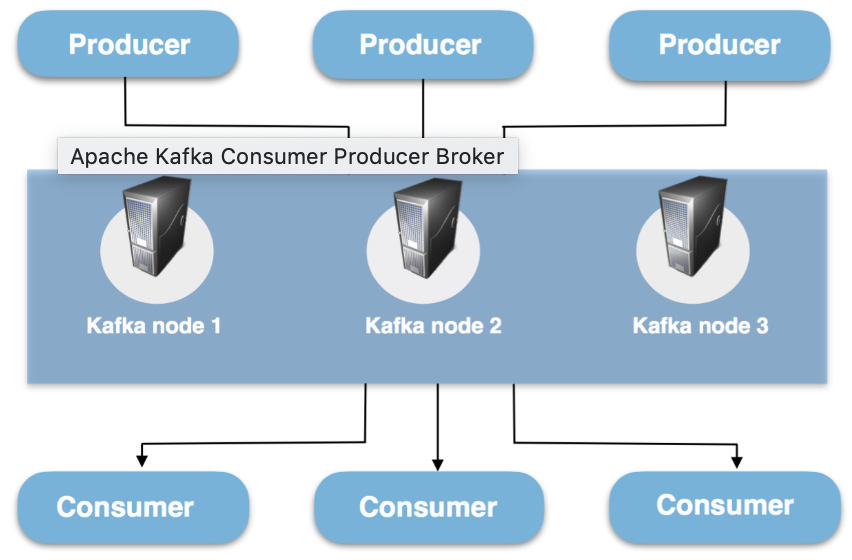
\includegraphics[width=80mm]{../kafkaCluster.png}
    \caption{Voorbeeld van een Kafka cluster}
    
\end{figure}

 Een topic kan je verdelen in verschillende partities. Dit wil zeggen dat je uw data kunt verdelen in ongeveer gelijke groepen (brokers). Iedere partitie kan dan staan voor een specifieke groep data binnen een topic zodat je niet alle berichten altijd moet overlopen. Dit principe van verschillende partities worden ook gebruikt bij traditionele databanken. Ook consumers kun je verdelen in verschillende partities, die samen één consumer-groep vormen. Door topics en consumers op deze manier op te delen, zorg je ervoor dat het mogelijk is dat meerdere consumers kunnen lezen van meerere partities in een topic. Dit heeft als positief gevolg dat je meer berichten kunt verwerken binnen een bepaalde tijd. 
 
 Ieder bericht binnen een partitie heeft een offset. Dit is een identifier, waardoor het mogelijk is om de berichten te ordenen. Normaal gezien als je als consumer je een subscriptie maakt op een topic, dan krijg je vanaf dit moment alle nieuwe berichten die binnen komen op de partitie waarop je een subscriptie hebt. Door een offset is het mogelijk om iets oudere berichten die op een partitie staan dan het moment dat je een subscriptie aangemaakt hebt, ook op te vragen. Op figuur 2.3 zie je een simpele voorstelling van een producer die berichten op een partitie van een topic plaatst. De cijfertjes stellen de offset voor van een bericht.
 \begin{figure}[h!]
     \centering
     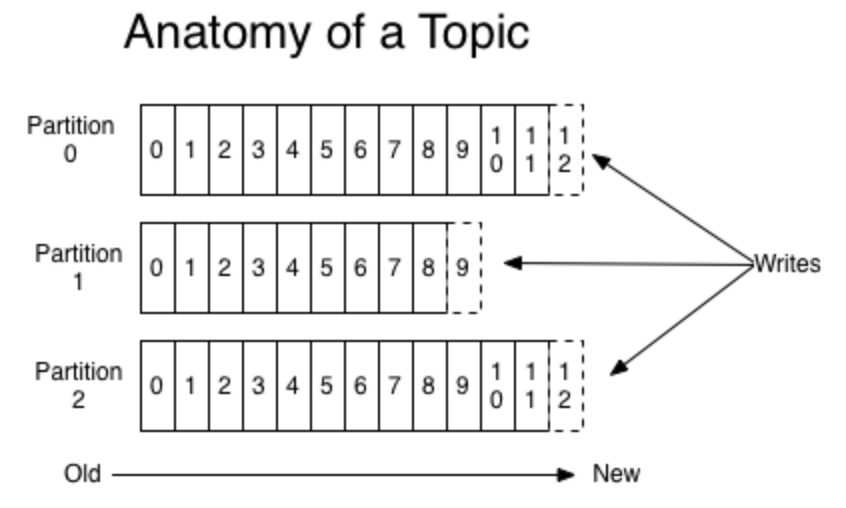
\includegraphics[width=80mm]{../kafkaOffset.png}
     \caption{Simpele voorstelling van de werking van een offset}
     
 \end{figure}

Het is al even vermeld, maar wat is nu eigenlijk een consumer-groep? Dit is een verzameling van verschillende consumers. Iedere consumer op zich leest van één specifieke partitie waardoor je het aantal berichten binnen één tijdseenheid kunt verhogen. Alle consumers binnen één groep lezen samen alle berichten die op een topic staan. Het opdelen van je topic in verschillende partities zorgt er dus niet voor dat je een deel van je data verliest. Mochten er meer consumers zijn dan dat er partities zijn, dan zitten er sommigen zonder werk. Omgekeerd, als er meer partities zijn dan consumers, dan krijgen consumers van verschillende partities berichten binnen.  Figuur 2.4 is een voorbeeld hoe een topic in verschillende servers kan opgedeeld worden en hoe consumers in consumer-groepen kunnen onderverdeeld worden. Je ziet dat de Kafka cluster in twee servers onderverdeelt is. Iedere server heeft twee partities. Er zijn 2 consumer-groepen, groep A bestaat uit twee consumers, groep B bestaat uit 4 consumers. Iedere partitie kan dus naar verschillende consumer-groepen berichten versturen, maar kan niet binnen dezelfde consumer-groep naar een andere consumer iets verzenden. 

 \begin{figure}[h!]
    \centering
    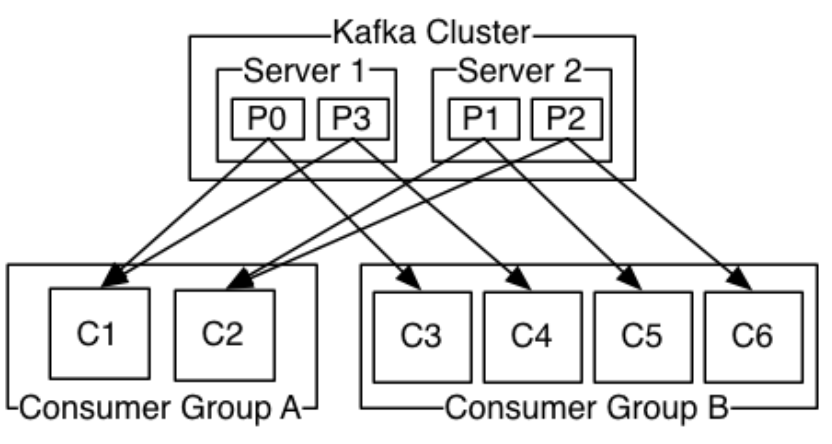
\includegraphics[width=80mm]{../kafkaConsumers.png}
    \caption{Wisselwerking tussen partities en consumer-groepen}
    
\end{figure}

\autocite{Sookocheff2015} en \autocite{Johansson2016}

\section{RabbitMq}

Een alternatief voor \emph{Kafka} is \emph{RabbitMq}. Dit is software waar men berichten kan plaatsen en ophalen op één of meerdere 'queues'. Ook hier heb je verschillende mogelijkheden van wat het formaat is van de berichten. Het kan zowel een gewone tekst zijn, als een Json-file. 

Wanneer een bericht van een queue wordt gelezen, dan wordt deze verwijderd van de queue. Het is dus niet mogelijk om later opnieuw hetzelfde bericht op te gaan vragen. De volledige queue kan ook een broker genoemd worden. Er zijn hier ook producers die data op de queue zetten, alsook consumers die een subscriptie kunnen maken op een queue. 



